%=========================================================================
% Autor: Matej Vadovič, 2023

\chapter{Úvod}
Každé zariadenie v sieti je identifikované pomocou IP adresy. Táto adresa je však pre človeka ťažko zapamätateľná a preto sa používajú doménové mená. Je však potrebné mať mechanizmus, ktorý umožní prevod doménového mena na IP adresu a naopak. Tento mechanizmus je DNS(Domain Name System). Pri komunikácií dvoch zaridení je potrebné poznať jeho IP adresu, ktorú odosielateť správy získa od DNS serveru pomocou DNS dotazu. Tieto dotazy klienti posielajú prostredníctvom DNS resolveru.

\textbf{DNS resolver} je lokálny agent, ktorý je zodpovedný za dotazovanie DNS serverov a spracovávanie odpovedí za účelom prekladu doménového mena/IP adresy alebo získavaním iných informácií spojených s doménovým menom. Umožňuje tak užívateľom rýchlešiu a jednoduchšiu navigáciu na internete.~\cite{RFC1035}

DNS resolver pracuje s distribuovaným, hierarchickým, stromovým doménovým priestorom. Tento priestor je rozdelený na \textbf{zóny}. Najvyšší bod hierarchie je \textbf{root DNS server}, ktorý obsahuje informácie o serveroch najvyššej úrovni (TLD - Top Level Domain), ktoré sú zodpovedné za správu domén pod nimi. Každá doména najvyššej úrovne má svojho správcu, ktorý je zodpovedný za správu domén pod ňou. Tento proces sa opakuje až na úroveň \textbf{autoritatívnych DNS serverov}, ktoré vykonávajú mapovanie názvu domény na adresu pre doménu danej organizácie~\cite{enwiki:1182387275}. Bližší popis doménového priestoru možno nájsť tu~\cite{RFC1034}.

Užívateľské programy interagujú s priestorom doménových mien pomocou resolveru. Resolver odpovedá na užívateľské dopyty informáciami, ktoré získa prostredníctvom dopytov na doménové servery a miestnu vyrovnávaciu pamäť. Na základe metód vyhľadávania možno DNS resolvery rozdeliť:
\begin{itemize}
    \item Iteratívny - dotazuje niekoľko DNS serverov v hierarchickej štruktúre doménového priestoru. Tento proces sa opakuje až kým resolver nedostane záznam z autoritatívneho servera pre danú doménu.
    \begin{figure}[!ht]
        \centering     % Center the image horizontally
        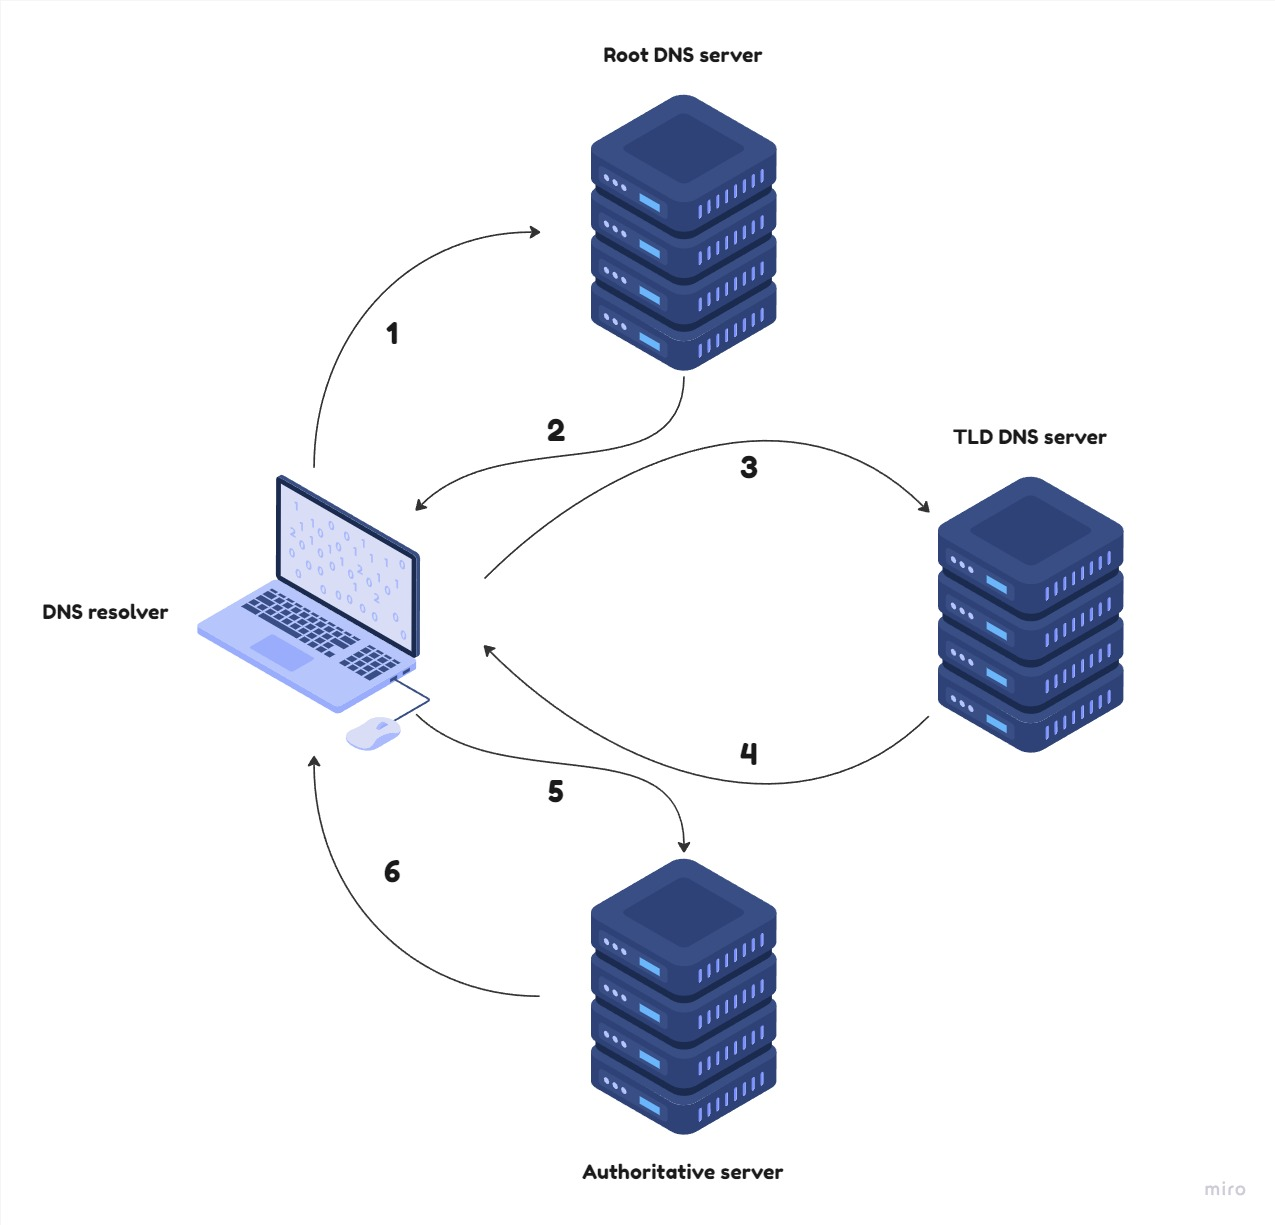
\includegraphics[width=0.6\textwidth]{obrazky-figures/Iterative.jpg}
        \caption{DNS resolver aplikujúci iteratívne dotazovanie}
        \label{fig:iterative-DNS-resolver}
    \end{figure}
    
    \item Ne-rekurzívny - dotazuje jeden DNS server, ktorý buď poskytne záznam z autoritatívneho serveru alebo čiastočnú odpoveď, bez toho, aby pokračoval v dotazovaní ďalších DNS serverov.
    
    \item Rekurzívny - dotazuje jeden DNS server, ktorý môže následne dotazovať ďalšie DNS servery. Tento proces na rozdiel od ne-rekurzívneho poskytuje kompletné riešenie pre danú doménu
    
    \begin{figure}[!ht]
        \centering     % Center the image horizontally
        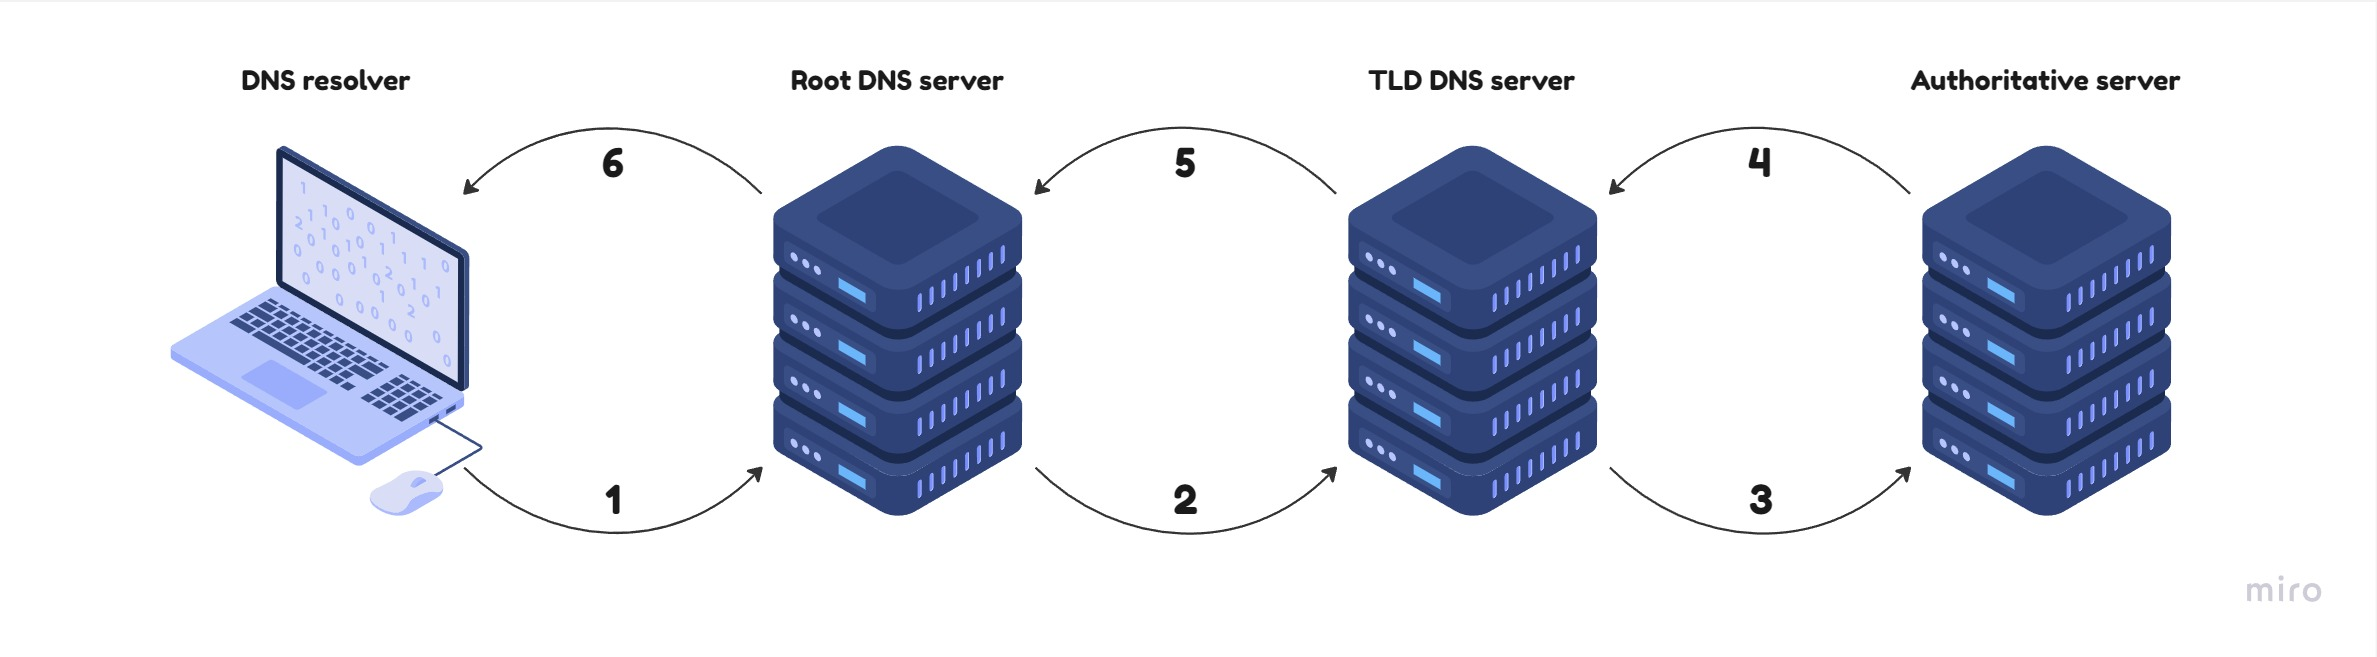
\includegraphics[width=0.6\textwidth]{obrazky-figures/Recursive.jpg}
        \caption{DNS resolver aplikujúci rekurzívne dotazovanie}
        \label{fig:recursive-DNS-resolver}
    \end{figure}
\end{itemize}

\chapter{Popis implementácie}
Program je implementovaný v jazyku C++ a pozostáva zo súborov dns.cpp(implementácia tried a funkcií) a dns.hpp(deklarácie tried a funkcií).

V rámci projektu som implementoval DNS resolver, ktorý podpuruje dotazovanie a tiež podporuje reverzné dotazovanie, teda preklad IP adresy na doménové meno, obe funkcie pre IPv4 aj IPv6 adresy.

Súčasťou projektu je aj testovací skript, ktorý testuje funkčnosť programu. Testovanie je popísané v kapitole~\ref{chap:testovanie}.

\section{Spracovanie argumentov}\label{sec:argumenty}
Pre spacovanie argumentov programu som použil knižnicu \textbf{getopt.h}. Táto knižnica umožňuje definovať argumenty programu a ich spracovanie. V prípade, že programu neboli predané argumenty, alebo boli predané argumenty, ktoré nie sú definované, program vypíše nápovedu a ukončí sa. V prípade, že boli predané argumenty, ktoré sú definované, program ich spracuje a uloží do štruktúry \textbf{s\_Arguments}. Táto štruktúra obsahuje všetky argumenty, ktoré program podporuje.

\noindent Argumenty a prepínače, ktoré program podporuje sú:
\begin{itemize}
    \item \textbf{-h} - vypíše nápovedu
    \item \textbf{-r} - rekurzívne dotazovanie
    \item \textbf{-x} - inverzné dotazovanie\footnote{Poznámka ku kombinácií argumentov -x a -6 - v prípade, že sú tieto argumenty kombinované, program vypíše varovnú hlášku o ignorovaní argumentu -6 a pokračuje v spracovaní.}
    \item \textbf{-6} - dotazovanie na IPv6 adresy\footnote{viď. poznámka pod čiarou č.1}
    \item \textbf{-s server} - doménové meno/IP adresa DNS servera, na ktorý sa bude dotazovať, povinný argument
    \item \textbf{-p port} - port DNS servera, na ktorý sa bude dotazovať, predvolená hodnota je 53
    \item \textbf{adresa} - doménové meno/IP adresa, o ktorú sa dotazujeme, povinný argument
\end{itemize}

\section{Komunikácia s DNS serverom}
Dotazovanie na DNS server je implementované v \texttt{main} funkcii. Rezolúciu domény DNS servera zabezpečuje funkcia \texttt{getaddrinfo}, ktorá podpuruje aj IPv6 adresy. Následne dochádza k vytvoreniu socketu pre komunikáciu protokolom UDP a vytvorenie dotazu. O zaslanie a prijatie dotazu na DNS server sa starajú funkcia \texttt{sendto()}, resp. \texttt{recvfrom()}. V prípade, že sa nepodarí zaslať dotaz, alebo prijať odpoveď(timeout je 3s), program vypíše chybovú hlášku a ukončí sa.
Zostavovaniu jednotlivých častí DNS dotazu sa venujú nasledujúce sekcie.

\subsection{DNS hlavička a dotaz}
Zostavenie DNS hlavičky a nastavenie dotazu je zabezpečené vo funkcii \texttt{create\_DNS\_query}. Tu dochádza k naplneniu hodnôt v štruktúre hlavičky \texttt{DNS\_header} a nastavenie dotazu v štruktúre \texttt{DNS\_question}. Štruktúry som vytváral podľa definícií v sekcií 4.1. Format v~\cite{RFC1035}.

\subsection{Prevod doménového mena na QNAME}
Funkcia \texttt{hostname\_to\_qname} vykonáva prevod doménového mena na QNAME(Query Domain Name). Táto funkcia rozdelí doménové meno na jednotlivé časti, ktoré sú oddelené znakom \uv{.} a pridá k nim dĺžku danej časti. Tento postup je opakovaný až kým nie je celé doménové meno prevedené na DNS formát.

\begin{gather*}
    \texttt{www.seznam.cz -> 3www5seznam2cz0}
\end{gather*}

\subsection{Reverzné dotazovanie}
V programe je podpora pre reverzné dotazovanie IPv4 aj IPv6 adries. Dve funkcie, a to \texttt{reverse\_ipv4\_address} a \texttt{reverse\_ipv6\_address}, slúžia na prevod IPv4 a IPv6 adries na doménové mená. 
\begin{gather*}
    \texttt{2001:4860:4860::8888 -> } \\ \texttt{8.8.8.8.0.0.0.0.0.0.0.0.0.0.0.0.0.0.0.0.0.6.8.4.0.6.8.4.1.0.0.2.ip6.arpa.}
\end{gather*}

\noindent Následne už stačí len zavolať funkciu \texttt{hostname\_to\_qname} a QNAME je pripravené.


\section{Spracovanie odpovede}
Spracovanie odpovede servera raidi funkcia \texttt{parse\_DNS\_response}. Táto funkcia spracuje DNS hlavičku a následne spracuje odpoveď na dotaz. V prípade, že kód odpovede nie je \texttt{0}, vypíše sa na stdout aj daný kód a pokračuje spracovanie. Následne sú spracované sekcie \texttt{Answer}, \texttt{Authority} a \texttt{Additional}. Na to slúži funkcia \texttt{parse\_section}, ktorá spracuje jednotlivé záznamy v sekcií.

\subsection{Podporované typy záznamov a ich obsah pri výpise}
Tu používam rovnaké označenia ako sú uvedené sekcií 3.2 RR definitions~\cite{RFC1035}, teda v anglickom jazyku, kde možno nájsť aj detailný popis jednotlivých typov záznamov a častí.
\begin{table}[!ht]
    \centering
    \begin{tabular}{|c|c|c|c|c|}
        \hline
        Name & TYPE & CLASS & TTL & ADDRESS \\
        \hline
    \end{tabular}
    \caption{Popis výpisu záznamu A}
\end{table}

\begin{table}[!ht]
    \centering
    \begin{tabular}{|c|c|c|c|c|}
        \hline
        Name & TYPE & CLASS & TTL & ADDRESS \\
        \hline
    \end{tabular}
    \caption{Popis výpisu záznamu AAAA}
\end{table}

\begin{table}[!ht]
    \centering
    \begin{tabular}{|c|c|c|c|c|}
        \hline
        Name & TYPE & CLASS & TTL & NSDNAME \\
        \hline
    \end{tabular}
    \caption{Popis výpisu záznamu NS}
\end{table}

\begin{table}[!ht]
    \centering
    \begin{tabular}{|c|c|c|c|c|c|c|}
        \hline
        Name & TYPE & CLASS & TTL &&&\\
        \hline
        MNAME & RNAME & SERIAL & REFRESH & RETRY & EXPIRE & MINIMUM\\
        \hline
    \end{tabular}
    \caption{Popis výpisu záznamu SOA}
\end{table}

\begin{table}[!ht]
    \centering
    \begin{tabular}{|c|c|c|c|c|}
        \hline
        Name & TYPE & CLASS & TTL & CNAME \\
        \hline
    \end{tabular}
    \caption{Popis výpisu záznamu CNAME}
\end{table}

\begin{table}[!ht]
    \centering
    \begin{tabular}{|c|c|c|c|c|}
        \hline
        Name & TYPE & CLASS & TTL & PTRDNAME \\
        \hline
    \end{tabular}
    \caption{Popis výpisu záznamu PTR}
\end{table}

\subsection{Prevod z QNAME na doménové meno}
Prevod z formátu QNAME na doménové meno je implementuje \texttt{qname\_to\_hostname}. Táto funkcia prechádza jednotlivé časti oddelené značkami. Funckia umožňuje aj prácu s kompresnými ukazateľmi, ktoré sú popísané v sekcií 4.1.4. Message compression~\cite{RFC1035}.

\begin{gather*}
    \texttt{3www5seznam2cz0 -> www.seznam.cz.}
\end{gather*}

\begin{figure}[!ht]
    \centering     % Center the image horizontally
    \includegraphics[width=0.6\textwidth]{obrazky-figures/query_ipv6.jpg}
    \caption{Dotazovanie o AAAA záznam pre doménové meno www.seznam.cz.}
    \label{fig:query_ipv6}
\end{figure}
\begin{figure}[!ht]
    \centering     % Center the image horizontally
    \includegraphics[width=0.6\textwidth]{obrazky-figures/rev_ipv6.jpg}
    \caption{Reverzné dotazovanie na IPv6 adresu.}
    \label{fig:rev_ipv6}
\end{figure}
\begin{figure}[!ht]
    \centering     % Center the image horizontally
    \includegraphics[width=0.6\textwidth]{obrazky-figures/compress_pointer_test 3.jpg}
    \caption{Ukážka spracovania odpovede, ktorá obsahuje viacero záznamov z rôznych kategórií a tiež veľa kompresných ukazateľov, sekcia 4.1.4. Message compression~\cite{RFC1035}.}
    \label{fig:compress_pointer_test_ipv6}
\end{figure}

\chapter{Testovanie}\label{chap:testovanie}
Pzthon skript \texttt{teest.py} sa stará o spustenie programu s rôznymi argumentami a následne porovnáva návratové hodnoty.

Pripravil som sadu testov v zložke \texttt{tests}, ktoré slúžia ako ukážka správneho výstupu. Pri tvorbe testov sade som použil nástroj dig a sledovanie paketov v prostredí Wireshark. Problém s testovaním sú premenlivé hodnoty, ktoré sa môžu vyskytnúť v odpovedi. Či už ide o poradie záznamov v jednotlivých sekciách alebo rozdielne hodnoty TTL alebo hodnôt v SOA zázname. Preto táto predpripravená sada slúži hlavne užívateľom na kontrolu správneho výstupu programu. V skripte je preto iba automatická kontrola návratovej hodnoty.



\chapter{Použitie}
Preklad programu je možné vykonať pomocou príkazu \texttt{make} v koreňovom adresári projektu. Program spustíte príkazom \texttt{./dns [-r] [-x] [-6] -s server [-p port] adresa}, pre detailný popis argumentov viz. sekcia~\ref{sec:argumenty}.

Testy možno spustiť pomocou príkazu \texttt{make test} v koreňovom adresári projektu.